%=========================
\chapter{La pile}
%=========================

\begin{center}
	
\includegraphics[width=7.553cm,height=4.357cm]{image/a2012Logique2eme-img011.png}
\end{center}
	

%===================
\section{Définition}
%===================
	
	\marginicon{pile}	
	Une \textbf{pile} est une collection d'éléments admettant 
	les fonctionnalités suivantes~:

	\begin{itemize}
		\item {
			on peut toujours ajouter un élément à la collection;}
		\item {
			seul le dernier élément ajouté peut être consulté ou enlevé;}
		\item {
			on peut savoir si la collection est vide.}
	\end{itemize}

	La pile (en anglais \textit{stack}) est donc une collection 
	de données de type \textit{dernier entré, premier sorti} (en
	anglais on dit «~LIFO~», c'est-à-dire \textit{last in first out}). 
	L'analogie avec la pile de dossiers sur un bureau
	est claire~: les dossiers sont déposés et retirés du sommet 
	et on ne peut jamais ajouter, retirer ou consulter un dossier 
	qui se trouve ailleurs dans la pile.
	
	\begin{center}
	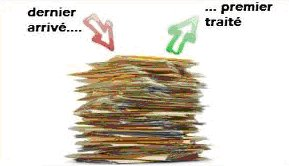
\includegraphics[width=7.553cm,height=4.357cm]{image/a2012Logique2eme-img012.jpg}
	\end{center}
	
	On ne peut donc pas parcourir une pile, ou consulter directement 
	le \textit{n}\textsuperscript{ième} élément. Les opérations permises
	avec les piles sont donc peu nombreuses, mais c'est précisément 
	là leur spécificité~: elles ne sont utilisées en
	informatique que dans des situations particulières où seules 
	ces opérations sont requises et utilisées. Paradoxalement,
	on implémentera une pile en restreignant des structures plus 
	riches aux seules opérations autorisées par les piles.
	
	Des exemples d'utilisations sont la gestion de la mémoire 
	par les micro-processeurs, l'évaluation des expressions
	mathématiques en notation polonaise inverse, la fonction 
	«~ctrl-Z~» dans un traitement de texte qui permet d'annuler
	les frappes précédentes, la mémorisation des pages web visitées 
	par un navigateur, etc. Nous les utiliserons aussi plus
	loin dans ce cours pour parcourir les arbres et les graphes.


%=====================================
\section{Implémentation orienté-objet}
%=====================================

	\subsection{Allure générale}
	%===========================
		
		Nous allons d'abord décrire l'allure générale de la 
		classe pile. Nous ne précisons pas encore les détails de
		l'implémentation, plusieurs possibilités existent, 
		que nous détaillerons à titre d'exercice.

		\cadre{
			\begin{pseudo}
				\Class{Pile<T>}
				\RComment T est le type des éléments de la pile
					\Private 
						\LComment {à détailler plus tard}
					\Public 
						\ConstrSign{Pile<T>}{}
						\RComment crée une pile vide
						\MethodSign{empiler}{élément~: T}{}
						\RComment ajoute un élément au sommet de la pile
						\MethodSign{sommet}{}{T}
						\RComment retourne la valeur de l'élément au sommet de la pile, sans le retirer
						\MethodSign{dépiler}{}{T}
						\RComment enlève et retourne l'élément au sommet
						\MethodSign{estVide}{}{booléen}
						\RComment indique si la pile est vide
				\EndClass
			\end{pseudo}
		}
		
	\subsection{Remarques~:}
	%=======================
		
		\begin{itemize}
			\item 
				Théoriquement, et dans la majorité des utilisations, la pile 
				est \textit{infinie}, c'est-à-dire qu'on peut y ajouter un
				nombre indéterminé d'éléments (comme c'était le cas pour la 
				classe Liste étudiée en 1\textsuperscript{ère} année). Dans
				certaines situations, on peut cependant imposer une capacité 
				maximale à la pile (en pratique, c'est le cas de la pile
				de dossiers dans un bureau, elle est forcément limitée par 
				la hauteur du plafond !). Nous aborderons ce cas particulier
				dans les exercices.
			\item 
				Lors de l'implémentation de la classe, il faudra songer à envoyer 
				un message d'erreur lorsqu'on utilise les méthodes
				\textit{sommet} et \textit{dépiler} si la pile est vide. 
				Si la pile possède une taille maximale, alors c'est
				\textit{empiler} qui doit générer un message d'erreur 
				lorsque la pile est pleine.
			\item
				Nous avons utilisé ici des noms de méthodes neutres indépendants 
				de tout langage de programmation. Dans la littérature
				anglaise, on trouvera souvent \textit{push}, \textit{top} et 
				\textit{pop} en lieu et place de \textit{empiler},
				\textit{sommet} et \textit{dépiler}.
		\end{itemize}
		

%==============================
\section{Exemple d'utilisation}
%==============================

	Afin d'illustrer l'utilisation de la classe Pile, nous donnons 
	pour exemple un algorithme qui lit une suite d'enregistrements d'un 
	fichier \textbf{fileIn} (de type \textbf{Info}) et les reproduit en 
	ordre inverse dans le fichier \textbf{fileOut}.
	
	\cadre{
		\begin{pseudo}
			\Module{inverserOrdre}{fileIn\In~: FichierEntrée d'Info, fileOut\Out~: FichierSortie d'Info}{}
				\Decl enr~: Info
				\Decl pile~: Pile<Info>
				\LComment {1\textsuperscript{ère} étape~: parcours du fichier et mise en pile}
				\Let pile \Gets \K{nouveau} Pile<Info>
				\Stmt fileIn.ouvrir( )
				\Let enr \Gets fileIn.lire( )
				\While{NON fileIn.EOF( )}
					\Stmt pile.empiler(enr)
					\Let enr \Gets fileIn.lire( )
				\EndWhile
				\Stmt fileIn.fermer( )
				\LComment{2\textsuperscript{e} étape~: vider la pile et écrire les éléments dans le fichier de sortie}
				\Stmt fileOut.ouvrir( )
				\While{NON pile.estVide( )}
					\Let enr \Gets pile.dépiler( )
					\Stmt fileOut.écrire(enr)
				\EndWhile
				\Stmt fileOut.fermer( )
			\EndModule
		\end{pseudo}
	}
	
	
%==================
\section{Exercices}
%==================

	\begin{Exercice}{Implémentation via une liste chainée}
		
		Détaillez l'implémentation de la classe pile en utilisant 
		comme attribut privé une liste chainée. Veillez à utiliser les
		méthodes qui permettent la gestion la plus efficace.
	\end{Exercice}

	\begin{Exercice}{La pile de taille finie}
		
		On envisage ici une pile dont la capacité est limitée~: elle 
		ne peut contenir au plus qu'un nombre donné d'éléments. On
		demande d'implémenter ce type de pile en utilisant un tableau. 
		Les attributs privés de la classe seront les suivants~:
		
		\cadre{
			\begin{pseudo}
				\Class{Pile<T>}
					\Private
						\Decl tab~: tableau de T 
						\RComment tableau (dynamique) contenant les éléments de la pile
						\Decl indSommet~: entier
						\RComment indice du sommet de la pile
						\Decl tailleMax~: entier
						\RComment taille maximale de la pile
					\EndClass
			\end{pseudo}
		}
		
		On remplira le tableau en ajoutant les éléments les uns à la 
		suite des autres et en retenant la position du dernier
		élément, qui correspondra à la valeur de l'attribut \textbf{indSommet}. 
		Cet attribut augmentera lorsqu'on ajoute un
		élément, et va décroître lorsqu'on en retire un.

		Détaillez l'implémentation des méthodes de la classe pile 
		correspondant à cette situation. Il faudra aussi
		adapter le constructeur, en lui donnant comme paramètre 
		la taille maximale de la pile.
	\end{Exercice}
	
	\begin{Exercice}{L'itinéraire retour}
		
		Un fichier \textbf{aller} contient la description d'un itinéraire. 
		Chaque enregistrement du fichier est une structure \textbf{étape} 
		contenant les champs \textbf{ville} (chaine) et \textbf{km} (réel). 
		Écrire un algorithme qui crée le fichier \textbf{retour} qui contiendra 
		-- au même format que \textbf{aller} -- la description de l'itinéraire retour.

		\bigskip

		\textbf{Exemple~:}
		
		\bigskip
		
		\begin{center}
		\tablefirsthead{}
		\tablehead{}
		\tabletail{}
		\tablelasttail{}
		\begin{supertabular}{|m{4.5cm}|m{2.0cm}|m{4.5cm}|m{2.0cm}|}
		\multicolumn{1}{m{4.5cm}}{{\itshape aller}} &
		\multicolumn{1}{m{2.0cm}}{{\itshape }} &
		\multicolumn{1}{m{4.5cm}}{{\itshape retour}} &
		\multicolumn{1}{m{2.0cm}}{{\itshape }} \\
		
		\multicolumn{1}{m{4.5cm}}{{ Bruxelles}} &
		\multicolumn{1}{m{2.0cm}}{{ 0}} &
		\multicolumn{1}{m{4.5cm}}{{ Amsterdam}} &
		\multicolumn{1}{m{2.0cm}}{{ 0}}\\
		
		\multicolumn{1}{m{4.5cm}}{{ Antwerpen}} &
		\multicolumn{1}{m{2.0cm}}{{ 40}} &
		\multicolumn{1}{m{4.5cm}}{{ Utrecht}} &
		\multicolumn{1}{m{2.0cm}}{{ 50}}\\
		
		\multicolumn{1}{m{4.5cm}}{{ Breda}} &
		\multicolumn{1}{m{2.0cm}}{{ 100}} &
		\multicolumn{1}{m{4.5cm}}{{ Breda}} &
		\multicolumn{1}{m{2.0cm}}{{ 120}}\\
		
		\multicolumn{1}{m{4.5cm}}{{ Utercht}} &
		\multicolumn{1}{m{2.0cm}}{{ 170}} &
		\multicolumn{1}{m{4.5cm}}{{ Anterpen}} &
		\multicolumn{1}{m{2.0cm}}{{ 180}}\\
		
		\end{supertabular}
	\end{center}

\end{Exercice}

